\section{Geometry of linear programming}

\begin{definition}
    A \emph{level curve} for a value $z$ of a function $f$ is the collection of points in $\mathbb{R}^n$  where the function $f$ remains constant and equals $z$.

    A \emph{hyperplane} is described as $H=\{x \in \mathbb{R}^n|a^Tx=b\}$. 

    An \emph{affine half-space} is represented as $H=\{x \in \mathbb{R}^n|a^Tx \leq b\}$. 
\end{definition}
Every inequality constraint defines an affine half-space within the variable space.
\begin{definition}
    The feasible region $x$  in any linear programming problem forms a \emph{polyhedron}, denoted as $P$. 

    A subset $S \subseteq \mathbb{R}^n$ is considered \emph{convex} if, for any pair $y^1,y^2 \in S$, the entire line segment connecting $y^1$ and $y^2$ is contained within $S$. 

    The line segment defined by $y^1$ and $y^2 $ in $ S$, encompassing all \emph{convex combinations} of $y^1$ and $y^2$, is denoted as:
    \[[y^1,y^2]=\{x \in \mathbb{R}^n|x=\alpha y^1+(1-\alpha)y^2 \land \alpha \in [0,1]\} \]
\end{definition}
\begin{property}
    A polyhedron $P$ is a convex set of $\mathbb{R}^n$. 
\end{property}
This occurs because each half-space is inherently convex, and the intersection of a finite number of convex sets likewise forms a convex set.

\begin{definition}
    A \emph{vertex} of $P$ is a point $P$ that cannot be represented as a convex combination of two other distinct points of $P$. 
\end{definition}
In terms of algebraic expression, a vertex is defined as:
\[x= \alpha y^1+(1-\alpha)y^2, \alpha \in [0,1], y^1,y^2 \in P \implies x=y^1 \lor x=y^2\]
\begin{property}
    A non-empty polyhedron $P=\{x \in \mathbb{R}^n|Ax=b,x \geq 0\}$ (in standard form) or $P=\{x \in \mathbb{R}^n|Ax=b,x \geq 0\}$ (in canonical form) possesses a finite number ($n \geq 1$) of vertices. 
\end{property}
\begin{definition}
    In the context of a problem $P$, a vector $d \in \mathbb{R}^n$ where $d \neq 0$ is considered an \emph{unbounded feasible direction of P} if, for any  point $x_0 \in P$, the ray defined as $\{x \in \mathbb{R}^n|x=x_0+\lambda d,\lambda \geq 0\}$ remains entirely within $P$.
\end{definition}
\begin{theorem}
    Each point $x$ within a polyhedron $P$ can be represented as a convex combination of its vertices $x^1,\dots,x^k$ and, if necessary, an unbounded feasible direction $d$ of $P$: 
    \[x=\alpha_1x^1+\dots+\alpha_kx^k+d\]
    Here, the coefficients $\alpha_i \geq 0$ fulfill the condition $\alpha_1+\dots+\alpha_k=1$. 
\end{theorem}
\begin{definition}
    A \emph{polytope} is a type of bounded polyhedron, which means it possesses only one unbounded feasible direction, and that direction is $d=0$. 
\end{definition}
Each point $x$ within a polytope $P$ can be represented as a convex combination of its vertices.
\begin{example}
    The point $x=\alpha_1x^1+\alpha_2x^2+\alpha_3x^3$ can also be expressed in the form $\alpha_1+\alpha_2+\alpha_3=1$ $(d=0)$. 
    \begin{figure}[H]
        \centering
        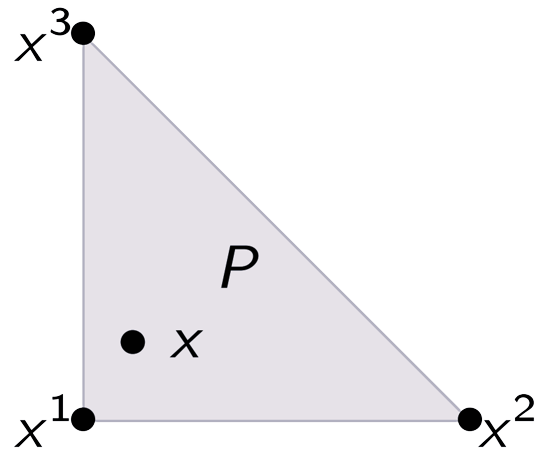
\includegraphics[width=0.2\linewidth]{images/polytope.png}
    \end{figure}
\end{example}
The following theorem is recognized as the Fundamental Theorem of Linear Programming.
\begin{theorem}
    Consider a linear programming problem $\min\{c^Tx|x \in P\}$, where $P \subseteq \mathbb{R}^n$ represents a non-empty polyhedron of feasible solutions (in standard or canonical form), one of the following scenarios must hold true:
    \begin{enumerate}
        \item There exists at least one optimal vertex within $P$.
        \item The value of the objective function is unbounded from below over $P$.
    \end{enumerate}
\end{theorem}
\begin{proof}[of case one]
    If $P$ contains an unbounded feasible direction $d$ such that $c^Td < 0$, it signifies that $P$ is unbounded, and the objective function values $z=c^Tx$ decrease indefinitely along the direction $d$. 
\end{proof}
\begin{proof}[of case two]
    If $P$ does not possess any unbounded feasible direction $d$ such that $c^Td < 0$, meaning that for all directions $d$, we have$c^Td \geq 0$, then any point within $P$ can be expressed as: 
    \[x=\sum_{i=1}^k{\alpha_ix^i + d}\]
    Here, $x^1,\dots,x^k$ are the vertices of $P$, $\alpha_i > 0$ with $\alpha_1+\dots+\alpha_k=1$, and $d = 0$, or $d$ represents an unbounded feasible direction.
    For any point $x \in P$, either $d = 0$ or $c^Td > 0$, which leads to the following inequality:
    \[c^Tx=c^T\left(\sum_{i=1}^{k}{\alpha_ix^i+d}\right)=\sum_{i=1}^{k}{\alpha_ic^Tx^i+c^Td}\geq\min_{i=1,\dots,n}{c^Tx^i}\]
    This is due to the fact that $\alpha_i > 0$ for any $i$, and $\alpha_1+\dots+\alpha_k=1$. 
\end{proof}
From this theorem, we can deduce that an interior point $x \in P$ cannot be an optimal solution. 
Furthermore, in an optimal vertex, all feasible directions lead to worse objective function values.
This theorem suggests that even though the variables can take fractional values, linear programming can be approached as a combinatorial problem.
Consequently, it is essential to investigate the vertices of the polyhedron of feasible solutions.
However, the number of vertices is finite but can often grow exponentially, making graphical methods practical only when $n \leq 3$. 
\begin{table}[H]
    \centering
    \begin{tabular}{cc}
    \hline
    \textbf{Type}              & \textbf{Example}                                                                                                   \\ \hline
    Unique optimal solution    & \begin{minipage}{.2\textwidth}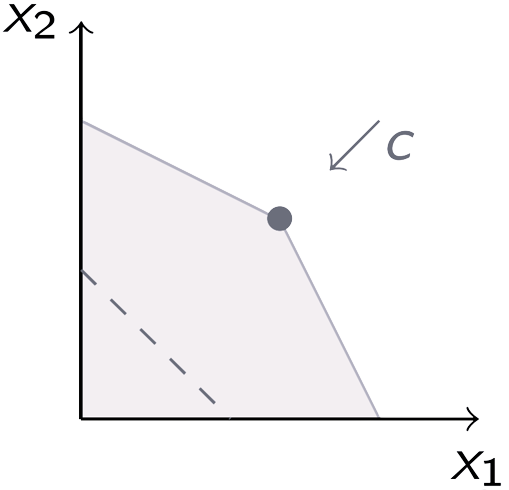
\includegraphics[width=\linewidth, height=30mm]{images/un.png}\end{minipage}         \\ 
    Multiple optimal solutions & \begin{minipage}{.2\textwidth}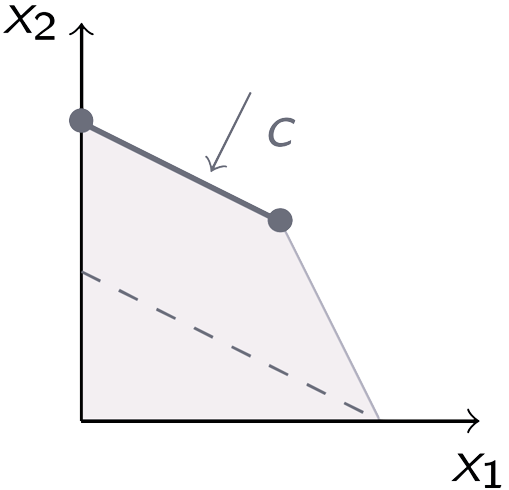
\includegraphics[width=\linewidth, height=30mm]{images/mul.png}\end{minipage}        \\
    Unbounded linear program   & \begin{minipage}{.2\textwidth}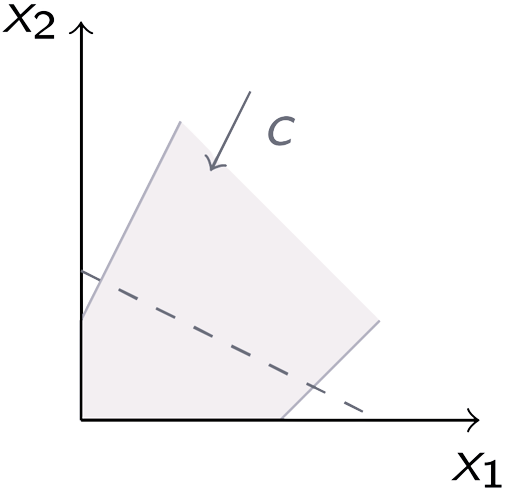
\includegraphics[width=\linewidth, height=30mm]{images/unb.png}\end{minipage}        \\
    Infeasible linear program  & \begin{minipage}{.2\textwidth}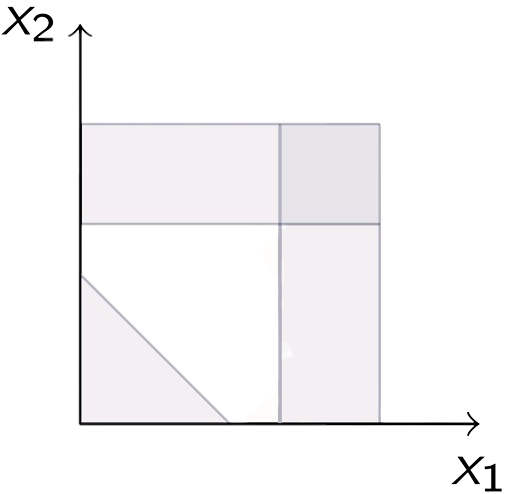
\includegraphics[width=\linewidth, height=30mm]{images/in.png}\end{minipage}         \\     
    \hline       
    \end{tabular}
\end{table}